%%%%%%%%%%%%%%%%%%%%%%%%%%%%%%%%%%%%%%%%%%%%%%%%%%%%%%%%%%%%%%%%%%%%%%%%%%%%
%    DO NOT TOUCH (just put your project_proposal.pdf in directory         %
% If the text fields are empty in the pdf, try print to pdf function which %
% can be seen as one of the printing options when trying to print a pdf.   %
% That writes a pdf that removes the fields and only keep the text.        % 
%%%%%%%%%%%%%%%%%%%%%%%%%%%%%%%%%%%%%%%%%%%%%%%%%%%%%%%%%%%%%%%%%%%%%%%%%%%%
\eprsec{Part 2. Project definition: approved Project Proposal}

This section contains the problem identification in the form of the complete approved Project Proposal, unaltered from the final approved version that appears on the AMS.

\addcontentsline{toc}{altsection}{1.\hspace{0.8em}Project description}
\addcontentsline{toc}{altsection}{2.\hspace{0.8em}Technical challenges in this project}
\addcontentsline{toc}{altsection}{3.\hspace{0.8em}Functional analysis}
\addcontentsline{toc}{altsection}{4.\hspace{0.8em}System requirements and specifications}
\addcontentsline{toc}{altsection}{5.\hspace{0.8em}Field conditions}
\addcontentsline{toc}{altsection}{6.\hspace{0.8em}Student tasks}

\mustcomplete{The approved Project Proposal included on the following pages is a PDF form whose
fields have not been flattened, so none of its filled-in content is rendered: the project
description, the technical challenges, the functional analysis, the requirement and specification
table, the field conditions and the student tasks all appear blank, and so do the title, student
number, study leader and the Feedback block. The fields are present in the file, but
\texttt{includepdf} does not draw form-field appearances. Appendix~4 requires Part~2 to be the
complete approved proposal, and an incomplete submission fails the project, so this must be fixed
before submission. To fix it: open
\texttt{2\_Project\_Definition/project\_proposal.pdf} in a PDF reader, use ``Print to PDF'' (which
flattens the fields into the page content), and replace that file with the printed copy. Then
rebuild and check that page~1 shows the title, the student number, the study leader and the
Feedback block, and that the later pages show the answers rather than empty boxes.}

\newpage

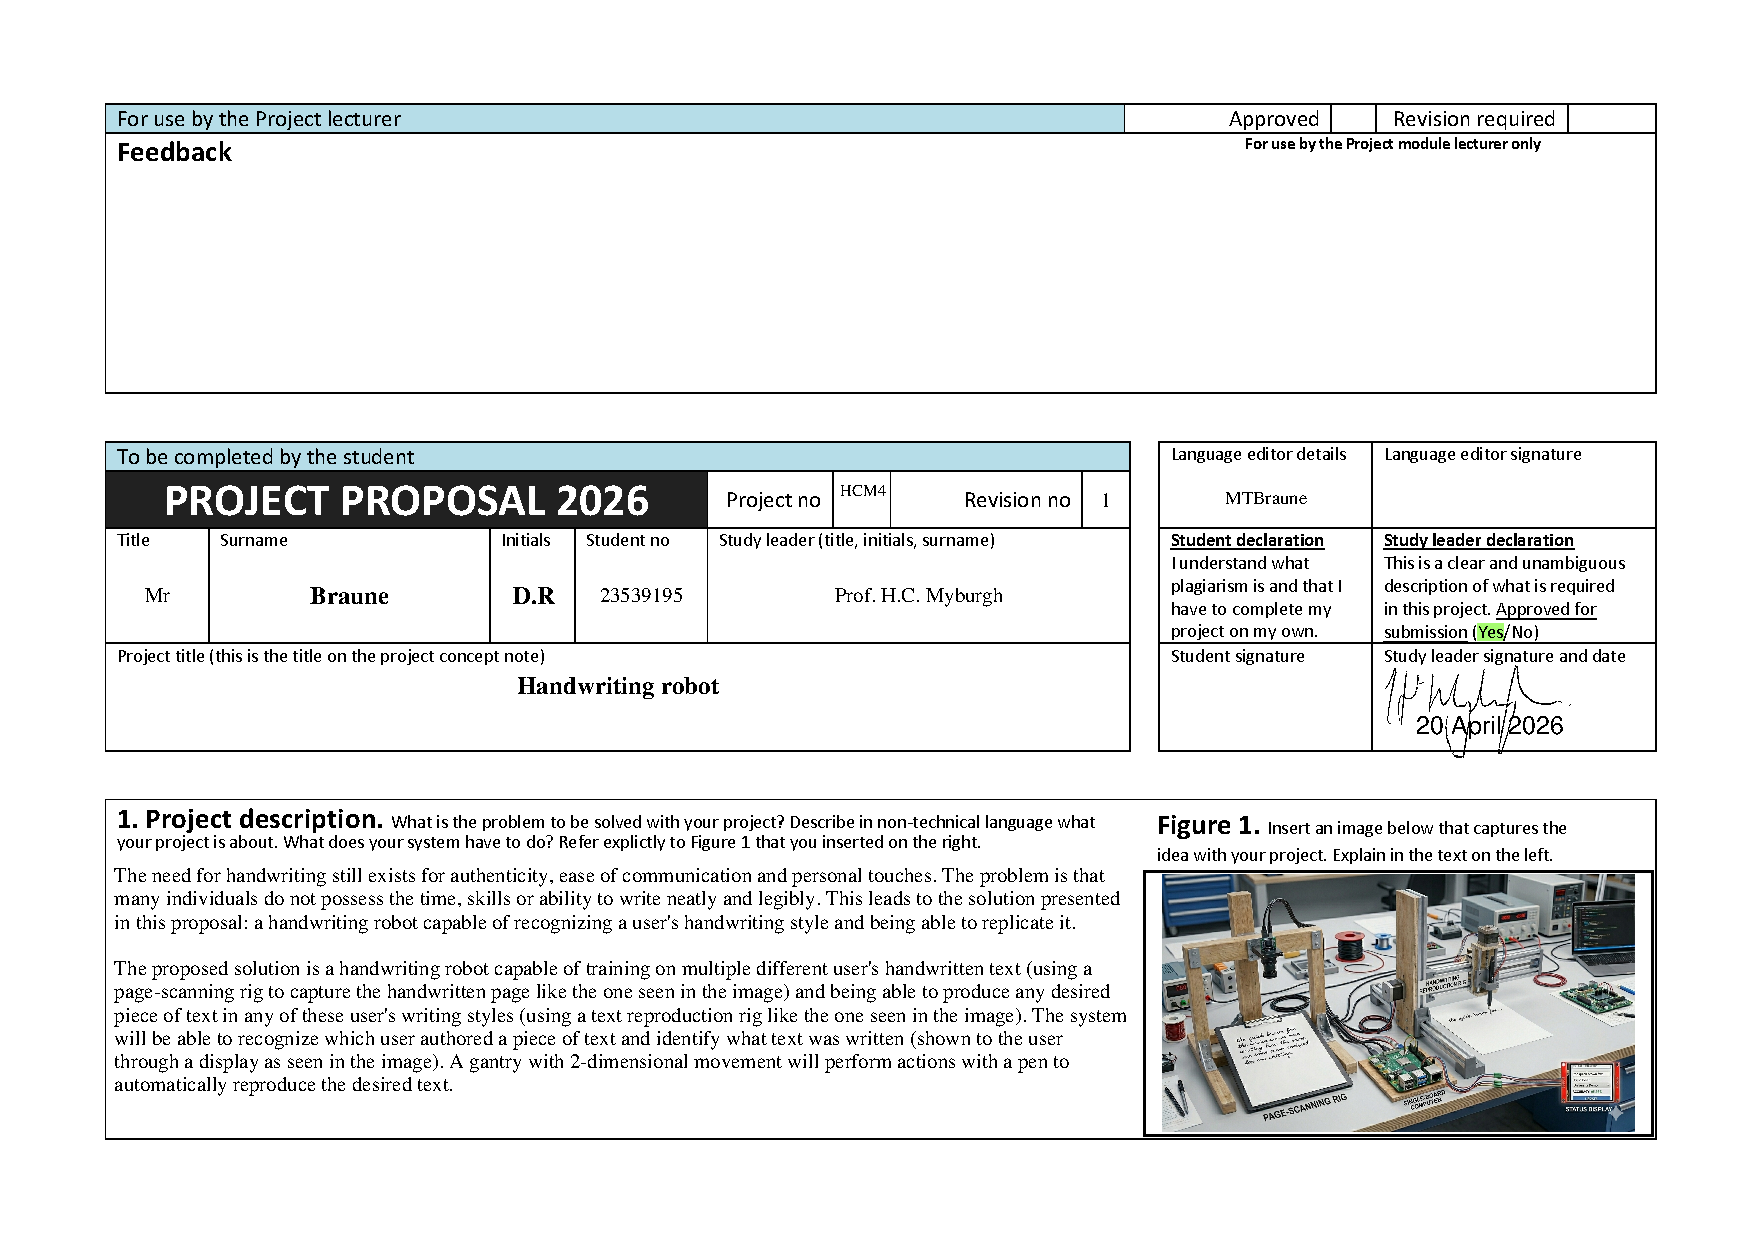
\includepdf[pages=-,landscape]{2_Project_Definition/project_proposal.pdf}
